\section{Experiments}
\subsection{Data Engines}
For each modality, specialized data engines are designed to curate data suitable for their respective training needs.



\noindent\textbf{Data engine for text prompt.} \ourmodel{} supports the integration of both detection and grounding data for training. Following~\cite{liu2023grounding, li2022grounded}, we utilize detection datasets Objects365~\cite{shao2019objects365}, OpenImages~\cite{krasin2017openimages}, along with the grounding dataset GoldG~\cite{kamath2021mdetr} for training. To enhance the text prompt capabilities of \ourmodel{}, we also make extensive use of pseudo-labeled data from image caption datasets and image classification datasets. Specifically, for image caption data in Conceptual Captions~\cite{sharma2018conceptual} and LAION400M~\cite{schuhmann2021laion} datasets, we use spaCy\footnote{\url{https://spacy.io/}} to extract noun chunks from image captions and use these noun chunks to prompt Grounding DINO~\cite{liu2023grounding} to get boxes. For image classification data in the Bamboo~\cite{zhang2022bamboo} dataset, we simply use the category of the current image to prompt Grounding DINO~\cite{liu2023grounding}. In total, we use 3.15M labeled images and 3.39M pseudo-labeled images for text prompt training.

\begin{table*}[t]
  \resizebox{\linewidth}{!}{
    \begin{tabular}{ccc|c|cccccccc|cc|c}
      \cline{1-15}
      \multirow{3}{*}{Method} & \multirow{3}{*}{\begin{tabular}[c]{@{}c@{}}Prompt \\ Type\end{tabular}} & \multirow{3}{*}{Backbone} & \begin{tabular}[c]{@{}c@{}}COCO-Val\\ Zero-Shot\end{tabular} & \multicolumn{8}{c|}{\begin{tabular}[c]{@{}c@{}}LVIS \\ Zero-Shot\end{tabular}}                                                                     & \multicolumn{2}{c|}{\begin{tabular}[c]{@{}c@{}}ODinW\\ Zero-Shot\end{tabular}} & \begin{tabular}[c]{@{}c@{}}Roboflow100\\ Zero-Shot\end{tabular} \\ \cline{4-15} 
                              &                                                                         &                           & val-80                                                       & \multicolumn{4}{c|}{minival-804}                                                   & \multicolumn{4}{c|}{val-1203}                                 & \multicolumn{2}{c|}{35val}                                                     & 100val                                                          \\ \cline{4-15} 
                              &                                                                         &                           & AP                                                           & AP            & $AP_f$         & $AP_c$         & \multicolumn{1}{c|}{$AP_{r}$}          & AP            & $AP_f$         & $AP_c$         & $AP_r$         & $AP_{avg}$                                & $AP_{med}$                               & $AP_{avg}$                                                         \\ \cline{1-15}
      GLIP-T~\cite{li2022grounded}                  & Text                                                                    & Swin-T                    & 46.7                                                         & 26.0          & 31.0          & 21.4          & \multicolumn{1}{c|}{20.8}          & 17.2          & 25.5          & 12.5          & 10.1          & 19.6                                   & 5.1                                   & -                                                               \\
      GLIP-L~\cite{li2022grounded}                  & Text                                                                    & Swin-L                    & 49.8                                                         & 37.3          & 41.5          & 34.3          & \multicolumn{1}{c|}{28.2}          & 26.9          & 35.4          & 23.3          & 17.1          & 23.4                                   & 11.0                                  & 8.6                                                             \\
      Grounding DINO~\cite{liu2023grounding}          & Text                                                                    & Swin-T                    & 48.4                                                         & 27.4          & 32.7          & 23.3          & \multicolumn{1}{c|}{18.1}          & -             & -             & -             & -             & 22.3                                   & 11.9                                  & -                                                               \\
      Grounding DINO~\cite{liu2023grounding}          & Text                                                                    & Swin-L                    & \textbf{52.5}                                                & 33.9          & 38.8          & 30.7          & \multicolumn{1}{c|}{22.2}          & -             & -             & -             & -             & 26.1                                   & 18.4                                  & -                                                               \\
      DetCLIPv2~\cite{yao2023detclipv2}               & Text                                                                    & Swin-T                    & -                                                            & 40.4          & 40.0          & 41.7          & \multicolumn{1}{c|}{36.0}          & -             & -             & -             & -             & -                                      & -                                     & -                                                               \\
      DetCLIPv2~\cite{yao2023detclipv2}               & Text                                                                    & Swin-L                    & -                                                            & 44.7          & 43.7          & 46.3          & \multicolumn{1}{c|}{43.1}          & -             & -             & -             & -             & -                                      & -                                     & -                                                               \\
      DINOv~\cite{li2023visual}                   & Visual-G                                                                & Swin-T                    & -                                                            & -             & -             & -             & \multicolumn{1}{c|}{-}             & -             & -             & -             & -             & 14.9                                   & 5.4                                   & -                                                               \\
      DINOv~\cite{li2023visual}                   & Visual-G                                                                & Swin-L                    & -                                                            & -             & -             & -             & \multicolumn{1}{c|}{-}             & -             & -             & -             & -             & 15.7                                   & 4.8                                   & -                                                               \\ \hline
      T-Rex2                  & Text                                                                    & Swin-T                    & \cellcolor{red!5}45.8                                        & \cellcolor{red!5}42.8          & \cellcolor{red!5}46.5          & \cellcolor{red!5}39.7          & \multicolumn{1}{c|}{\cellcolor{red!5}37.4}          & \cellcolor{red!5}34.8          & \cellcolor{red!5}41.2          & \cellcolor{red!5}31.5          & \cellcolor{green!5}29.0          & \cellcolor{green!5}18.0                                   & \cellcolor{green!5}4.7                                   & \cellcolor{green!5}8.2                                                             \\
      T-Rex2                  & Visual-G                                                                & Swin-T                    & \cellcolor{red!5}38.8                                        & \cellcolor{red!5}37.4          & \cellcolor{red!5}41.8          & \cellcolor{red!5}33.9          & \multicolumn{1}{c|}{\cellcolor{red!5}29.9}          & \cellcolor{red!5}\underline{34.9}          & \cellcolor{red!5}41.1          & \cellcolor{red!5}30.3          & \cellcolor{green!5}\underline{32.4}          & \cellcolor{green!5}\underline{23.6}                                   & \cellcolor{green!5}\underline{17.5}                                  & \cellcolor{green!5}\underline{17.4}                                                            \\ \hline
      T-Rex2                  & Text                                                                    & Swin-L                    & \cellcolor{red!5}\underline{52.2}                                        & \cellcolor{red!5}\textbf{54.9} & \cellcolor{red!5}\textbf{56.1} & \cellcolor{red!5}\textbf{54.8} & \multicolumn{1}{c|}{\cellcolor{red!5}\textbf{49.2}} & \cellcolor{red!5}\textbf{45.8} & \cellcolor{red!5}\textbf{50.2} & \cellcolor{red!5}\textbf{43.2} & \cellcolor{green!5}42.7          & \cellcolor{green!5}22.0                                   & \cellcolor{green!5}7.3                                   & \cellcolor{green!5}10.5                                                            \\
      T-Rex2                  & Visual-G                                                                & Swin-L                    & \cellcolor{red!5}46.5                                        & \cellcolor{red!5}47.6          & \cellcolor{red!5}49.5          & \cellcolor{red!5}46.0          & \multicolumn{1}{c|}{\cellcolor{red!5}45.4}          & \cellcolor{red!5}45.3          & \cellcolor{red!5}49.5          & \cellcolor{red!5}42.0          & \cellcolor{green!5}\textbf{43.8} & \cellcolor{green!5}\textbf{27.8}                          & \cellcolor{green!5}\textbf{20.5}                         & \cellcolor{green!5}\textbf{18.5}                                                   \\ \hline
      \end{tabular}}
  \caption{\textbf{One suit of weights} for zero-shot object detection. \textcolor{red!25}{Red} denotes regions where text prompt excels over visual prompt, while \textcolor{green!45}{green} signifies regions favoring visual prompts.}
  \vspace{-1.5em}
  \label{tab:main_result}
  \end{table*}

\noindent\textbf{Data engine for visual prompt.} The training process for visual prompts is to use a portion of the GT box or its center point in the current image as the input. Thus we can leverage established detection datasets including Objects365~\cite{shao2019objects365}, OpenImages~\cite{krasin2017openimages}, HierText~\cite{long2022towards}, CrowdHuman~\cite{shao2018crowdhuman} for the initial training. Meanwhile, to make the data for visual prompt sufficiently diversified, we constructed a data engine to harvest data from SA-1B~\cite{kirillov2023segment}.  This data engine operates through a self-training loop, comprising two phases: \textbf{1) Initial training stage}: In this stage, we first train an initial version of \ourmodel{} with only visual prompt modality on the aforementioned datasets, endowing it with preliminary capabilities for interactive object detection. \textbf{2) Annotation stage}: With the initial model, we then utilize it to annotate the data in SA-1B. SA-1B has tremendous boxes for objects at all granularity. However, the box has no semantic labels, which is not suitable for object detection training. Thus, we employ TAP~\cite{pan2023tokenize} to annotate each box with a category name from a dictionary of 2560 classes. We then adopt the following filtering strategy: if an image has at least one category with a number of instances greater than a certain threshold, it is reserved. However in SA-1B, not all objects have boxes, so we use the original GT box as the interactive visual prompt input and use the initial \ourmodel{} to annotate the missing labeled boxes. In total, we use 2.4M labeled images and 0.65M pseudo-labeled images for visual prompt training.



  \begin{table*}[h]
    \resizebox{\linewidth}{!}{
      \begin{tabular}{ccc|c|cccccccc|cc|c}
        \cline{1-15}
        \multirow{3}{*}{Method} & \multirow{3}{*}{\begin{tabular}[c]{@{}c@{}}Prompt \\ Type\end{tabular}} & \multirow{3}{*}{Backbone} & \begin{tabular}[c]{@{}c@{}}COCO-Val\\ Zero-Shot\end{tabular} & \multicolumn{8}{c|}{\begin{tabular}[c]{@{}c@{}}LVIS \\ Zero-Shot\end{tabular}}                                                                     & \multicolumn{2}{c|}{\begin{tabular}[c]{@{}c@{}}ODinW\\ Zero-Shot\end{tabular}} & \begin{tabular}[c]{@{}c@{}}Roboflow100\\ Zero-Shot\end{tabular} \\ \cline{4-15} 
                                &                                                                         &                           & val-80                                                       & \multicolumn{4}{c|}{minival-804}                                                   & \multicolumn{4}{c|}{val-1203}                                 & \multicolumn{2}{c|}{35val}                                                     & 100val                                                          \\ \cline{4-15} 
                                &                                                                         &                           & AP                                                           & AP            & $AP_f$         & $AP_c$         & \multicolumn{1}{c|}{$AP_{r}$}          & AP            & $AP_f$         & $AP_c$         & $AP_r$         & $AP_{avg}$                                & $AP_{med}$                               & $AP_{avg}$                                                         \\ \cline{1-15}
        T-Rex2                  & Visual-I (Box)                                                          & Swin-T                    & 56.6                                                         & 59.3          & 54.6          & 63.5          & \multicolumn{1}{c|}{64.4}          & 62.6          & 57.3          & 63.7          & 71.9          & 37.7                                   & 39.3                                  & 30.6                                                            \\
        T-Rex2                  & Visual-I (Box)                                                          & Swin-L                    & 58.5                                                         & 62.5          & 57.9          & 66.1          & \multicolumn{1}{c|}{70.1}          & 65.8          & 61.2          & 67.3          & 72.6          & 39.7                                   & 38.1                                  & 30.2                                                            \\
        T-Rex2                  & Visual-I (Point)                                                        & Swin-T                    & 54.3                                                         & 57.4          & 52.1          & 62.3          & \multicolumn{1}{c|}{63.2}          & 60.0          & 54.5          & 60.9          & 68.8          & 34.8                                   & 34.9                                  & 27.7                                                            \\
        T-Rex2                  & Visual-I (Point)                                                        & Swin-L                    & 56.8                                                         & 60.6          & 56.4          & 64.2          & \multicolumn{1}{c|}{65.3}          & 63.8          & 59.1          & 65.1          & 71.1          & 37.5                                   & 35.7                                  & 27.8                                                            \\ \hline
        \end{tabular}}
    \caption{\textbf{One suit of weights} for interactive object detection.}
    \label{tab:main_result_2}
    \end{table*}

\subsection{Model Details}
\ourmodel{} is built upon DINO~\cite{zhang2022dino}. We utilize Swin Transformer~\cite{liu2021swin} as the vision backbone, followed by six layers of transformer encoder layers. We use CLIP-B~\cite{clip} as the text encoder and fine-tune it. For the visual prompt encoder, we stack three layers of deformable cross-attention layer and set the hidden dimension of the feed-forward layer to 1024. We use AdamW~\cite{loshchilov2017decoupled} as the optimizer and set the learning rate to 1e-5 for backbone and text encoder, and 1e-4 for all other modules.

\subsection{Settings and Metrics}
For the object detection task, we evaluate in zero-shot setting, i.e. \ourmodel{} will not be trained on evaluation benchmarks. We report the AP metric on COCO~\cite{lin2014microsoft}, LVIS~\cite{gupta2019lvis}, ODinW~\cite{li2022elevater} and Roboflow100~\cite{ciaglia2022roboflow}. The COCO dataset encompasses 80 common categories. In contrast, the LVIS dataset is characterized by a long-tailed category distribution with 1203 categories. These categories are further segmented into three distinct groups: frequent, common, and rare, with a ratio of \texttt{405:461:337} for the val split, and \texttt{389:345:70} for the minival split~\cite{kamath2021mdetr}. The ODinW and Roboflow100 datasets contain 35 and 100 datasets collected from Roboflow\footnote{https://universe.roboflow.com/}, respectively, covering a variety of scenarios including aerial, video games, underwater, documents, real world, \etc., with long-tailed categories.

We compare several different evaluation protocols for \ourmodel{} under different workflows.

\textbf{Text}: In this protocol, we use all the category names of the benchmark as text prompt inputs, consistent with the previous open-vocabulary object detection setting.

\textbf{Visual-G (Generic)}: In this protocol, \ourmodel{} works on the generic visual prompt workflow. We extract visual prompt embeddings from the training set images of each benchmark for each category. Taking COCO as an example, we first randomly sample  $N$ images for each category that has at least one instance of that category. Next, we extract $N$ visual embeddings for each category using the GT box of each image as input for visual prompting. Subsequently, we compute the average of these $N$ embeddings for each category. These averaged visual embeddings (a total of 80 embeddings) will be used for evaluation. By default, $N$ is set to 16. For each test image, we will repeat this process.

\textbf{Visual-I (Interactive)}: In this protocol, \ourmodel{} works on the interactive visual prompt workflow. Given a test image, suppose it has M categories, then for each category, we randomly select one GT box (or convert it to its center point) in the current image as the visual prompt input for this category. This protocol is relatively easier than Visual-G as we know the category of the test set images in advance, as well as being provided with a GT box. However, despite its simplicity, interactive object detection boasts a wide range of application scenarios, including automatic annotation, object counting, \etc.


\subsection{Zero-Shot Generic Object Detection}
In this study, we explore the zero-shot object detection capabilities of \ourmodel{} across four distinct benchmarks: COCO, LVIS, ODinW, and Roboflow100. The term \textit{zero-shot} refers to the methodological approach where the evaluation benchmarks were not exposed to the model during its training phase, possibly encompassing novel categories and image distributions. As shown in Tab. \ref{tab:main_result}, we observe that text prompt and visual prompt can cover different scenarios respectively. Text prompt demonstrates superior performance in scenarios with relatively common categories. For instance, under the generic visual prompt and Swin-T backbone setting, text prompts surpass visual prompts by a margin of 7 AP points on COCO (80 categories). Similarly, in LVIS-minival (804 categories), text prompts achieve a 5.4 AP point advantage over visual prompts. Conversely, in scenarios characterized by long-tailed distributions, visual prompts exhibit a more robust performance compared to text prompts. Specifically, on LVIS-val (1203 categories), visual prompt leads by 3.4 AP points in the rare group, and by 5.6 AP points on ODinW as well as 9.2 AP points on Roboflow100, underscoring its efficacy in handling less common objects.

\begin{figure}[t]
\centering
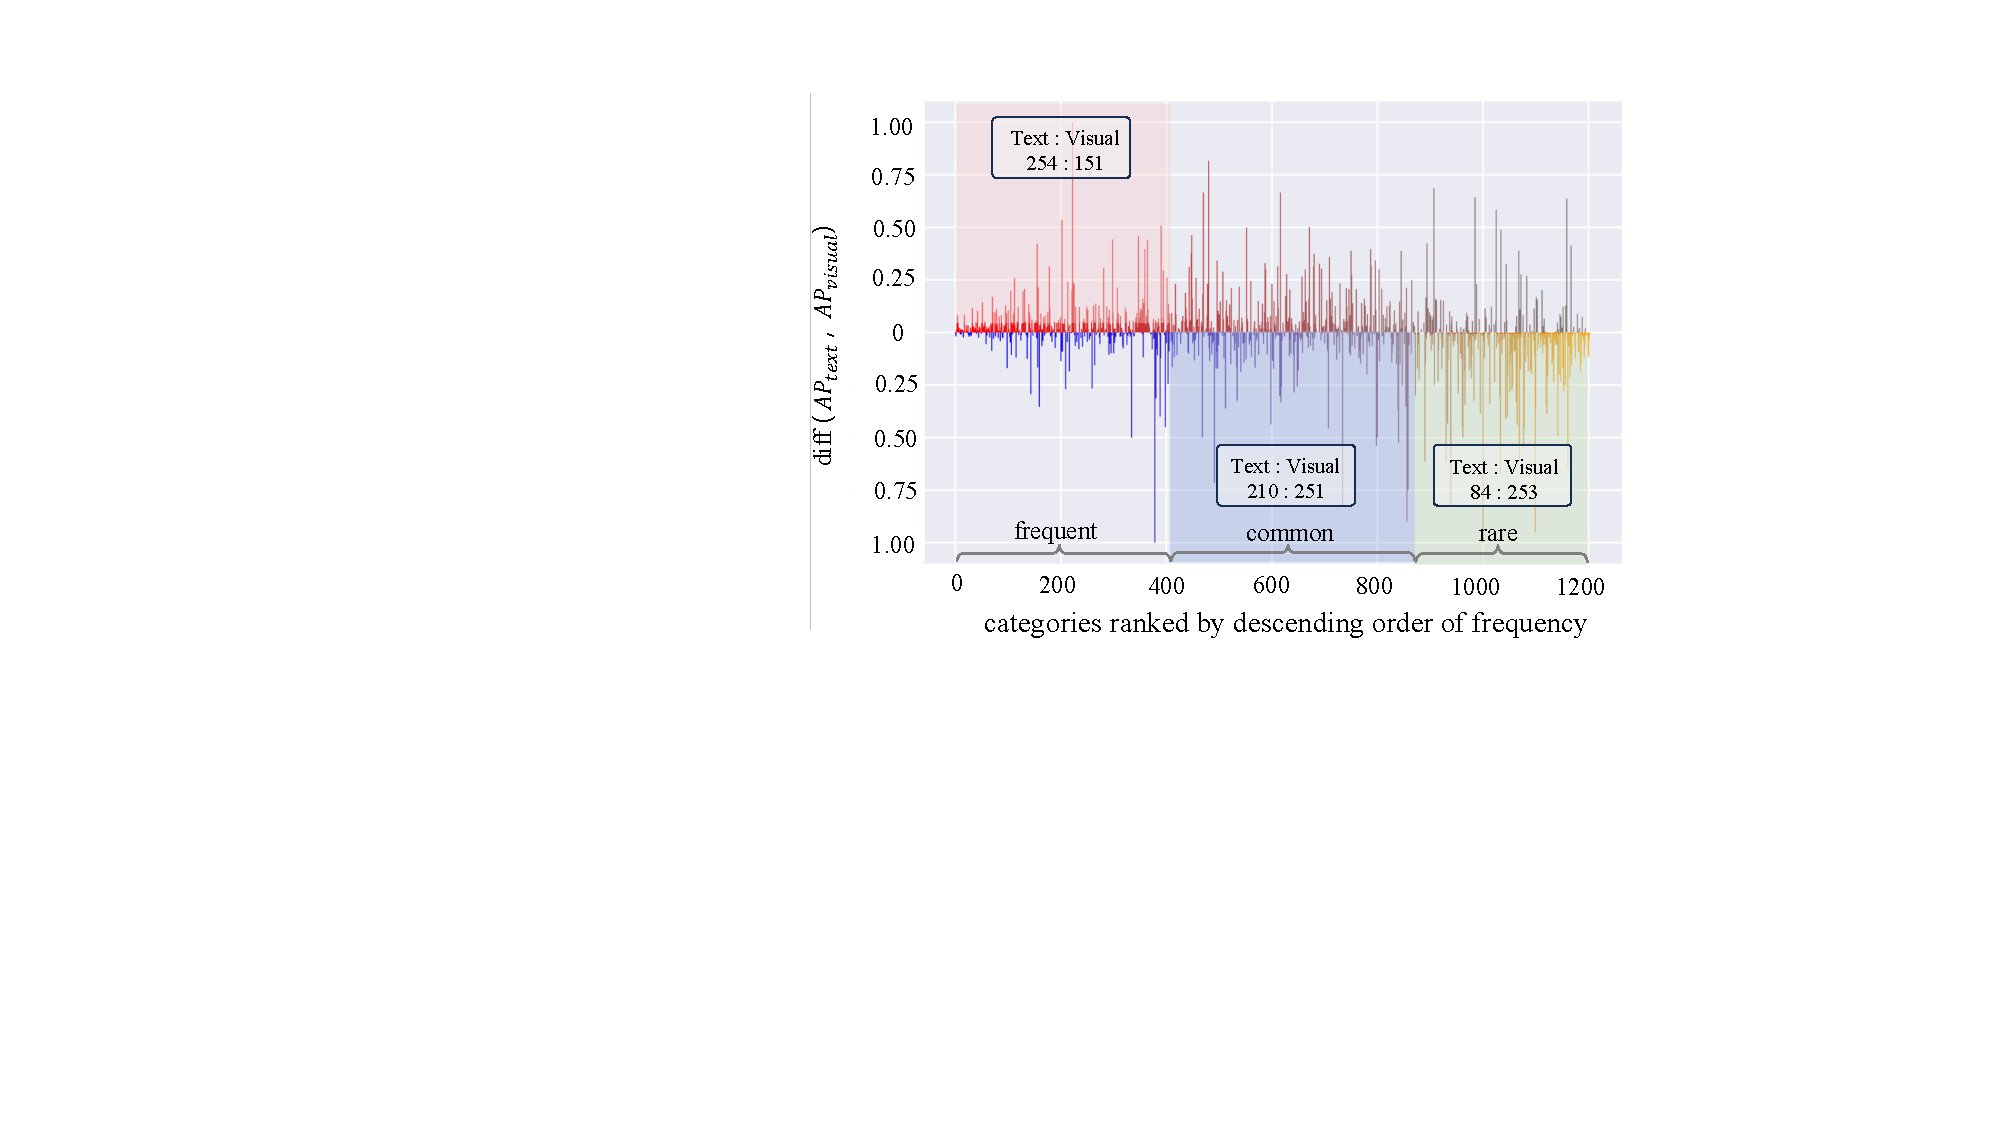
\includegraphics[width=1\linewidth]{images/text_visual_diff.pdf}\vspace{-1mm}
\caption{Compare the performance difference between text prompt and visual prompt on the long-tailed dataset LVIS-val. The vertical axis is the difference between the AP of text prompts and visual prompts on each category. The horizontal axis shows the categories of LVIS in descending order of their frequency of occurrence in the text prompt training data. \texttt{Text:Visual} refers to the number of times each has won in the current interval.}
\label{fig:lvis_results} 
\end{figure}

In Fig. \ref{fig:lvis_results}, we show the per-category AP difference between visual prompt and text prompt on the LVIS benchmark. We rank the categories of the LVIS dataset in descending order of their frequency of occurrence in the training set. Our analysis shows that text prompts perform better in recognizing common categories with higher occurrence frequencies. In contrast, visual prompts excel in identifying rarer categories as the frequency decreases. This indicates that text prompts are suited for common concepts, while visual prompts are more effective for rare categories. 


\begin{table}[]
  \centering
  \resizebox{0.8\columnwidth}{!}{%
   \begin{tabular}{c|c|c}
\hline
\multirow{2}{*}{Method} & \begin{tabular}[c]{@{}c@{}}FSC147\\ test\end{tabular} & \begin{tabular}[c]{@{}c@{}}FSCD-LVIS\\ test\end{tabular} \\ \cline{2-3} 
                        & MAE                                                   & AP                                                       \\ \hline
FamNet~\cite{ranjan2021learning}                  & 22.08                                                 & -                                                        \\
Counting-DETR~\cite{nguyen2022few}           &                                                       & 22.66                                                    \\
BMNet+~\cite{shi2022represent}                  & 14.62                                                 & -                                                        \\
CountTR~\cite{liu2022countr}                 & 11.95                                                 & -                                                        \\
T-Rex~\cite{jiang2023t}                   & \textbf{8.72}                                         & 40.32                                                    \\ \hline
T-Rex2                  & 10.94                                                 & \textbf{43.35}                                           \\ \hline
\end{tabular}}
\caption{Few-shot object counting results on FSC147~\cite{ranjan2021learning} and FSCD-LVIS~\cite{nguyen2022few} datasets.}
\label{tab:counting}
\end{table}

\subsection{Zero-Shot Interactive Object Detection}
\ourmodel{} also showcases strong interactive object detection capabilities. As shown in Tab. \ref{tab:main_result_2}, the interactive visual prompt significantly outperforms both text prompt and generic visual prompt strategies. However, this comparison may not be entirely equitable, as under the Visual-I setting we have the prior about the categories present in the test image. To provide more insight, we evaluate \ourmodel{} on the few-shot object counting task. In this task~\cite{jiang2023t, nguyen2022few, shi2022represent, liu2022countr}, each test image will be provided with three visual exemplar boxes of the target object and requires to output the number of the target object. We evaluate on FSC147~\cite{ranjan2021learning} and FSCD-LVIS~\cite{nguyen2022few} datasets. Both datasets comprise scenes with densely populated small objects. Specifically, FSC147 typically features single-target scenes, where generally only one type of object is present per image, whereas FSCD-LVIS mainly includes multi-target images. We report the Mean Average Error (MAE) metric for FSC147 and the AP metric for FSCD-LVIS. Following previous work~\cite{jiang2023t}, we use the visual exemplar boxes as the interactive visual prompt. As shown in Tab. \ref{tab:counting}, \ourmodel{} achieves competitive results compared with the previous SOTA algorithm T-Rex. While not matching T-Rex in terms of MAE, \ourmodel{} performs better than T-Rex in terms of AP, which measures the overall detection accuracy. This result suggests that \ourmodel{}’s interactive capabilities are highly capable in dense and small object scenarios.

\subsection{Ablation Experiments}
\noindent\textbf{Ablation of naive joint training.} As demonstrated in Tab. \ref{tab:synergy_ab} (first two rows), the general detection capability of the visual prompt is notably poor (14.0 AP on COCO and 15.3 AP on LVIS-val) when the two prompt modalities are trained separately. The core of the issue lies in the diversity and variance of visual data. For example, when the model is trying to understand what makes a \texttt{chair} when every example the model sees is drastically different from the last. Without a consistent context, it is challenging for the model to form a general concept solely with visual prompts. Upon joint training (second two rows in Tab. \ref{tab:synergy_ab}), the efficacy of visual prompts significantly improves. This improvement suggests that the combination of textual context with visual data helps the model form more stable and generalizable representations. However, the naive joint training without explicit alignment between the two prompts somewhat reduce the effectiveness of text prompts, as both AP on COCO and LVIS dropped.


The observed decline in text prompt capability could be due to the added complexity of multitask learning. We use t-SNE~\cite{van2008visualizing} to visualize the distribution of text prompt and visual prompt embeddings in Fig. \ref{fig:tsne_noalign}.
We find that the corresponding text prompt and visual prompt embeddings are separated in the feature space, instead of gathered. Therefore the region feature cannot be simultaneously aligned to both the text prompt and the visual prompt, thus making the learning process more challenging.

\begin{figure}[t]
\centering
\begin{subfigure}[b]{0.22\textwidth}
    \centering
    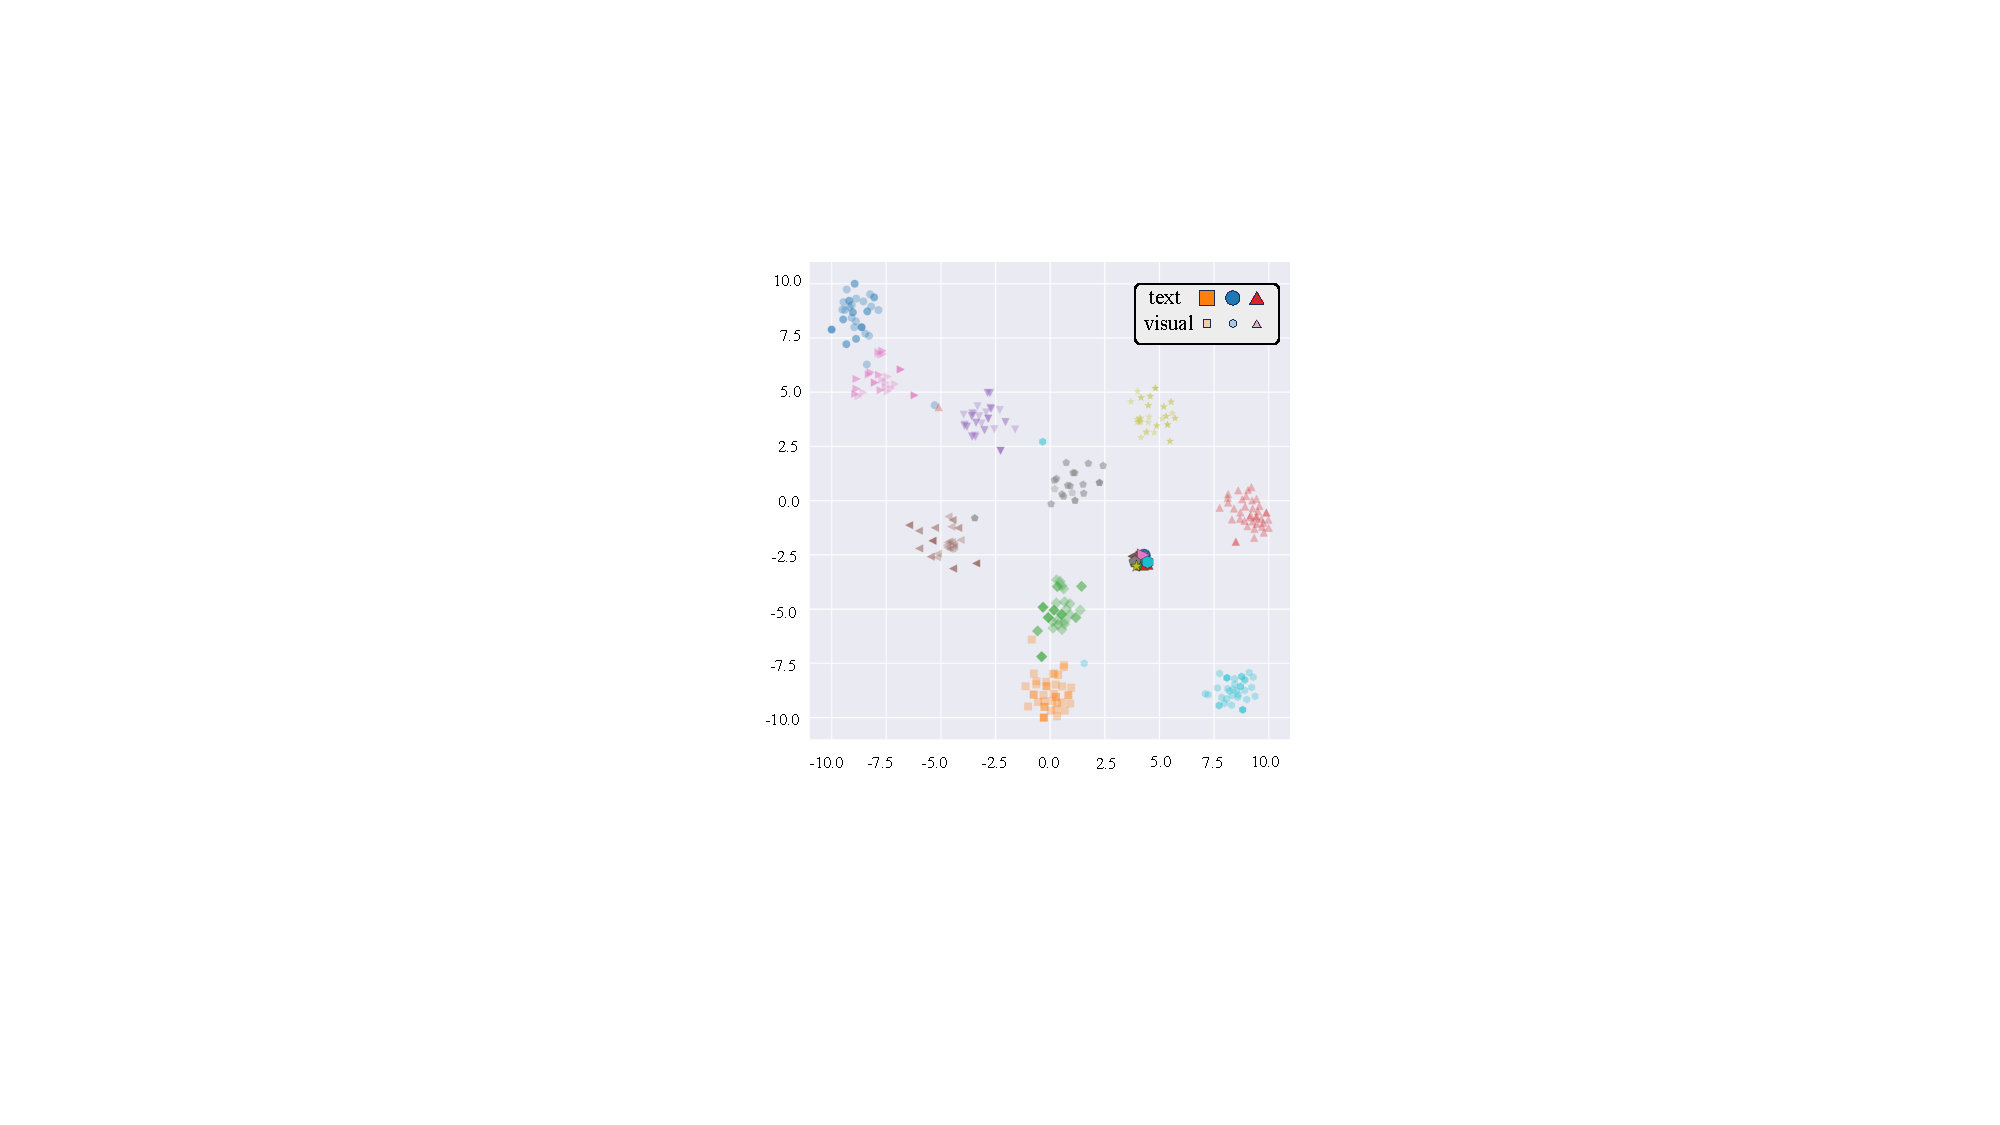
\includegraphics[width=\textwidth]{images/tsne_noalign.pdf}
    \caption{w/o contrastive align}
    \label{fig:tsne_noalign}
\end{subfigure}
\hspace{5pt}
\begin{subfigure}[b]{0.22\textwidth}
    \centering
    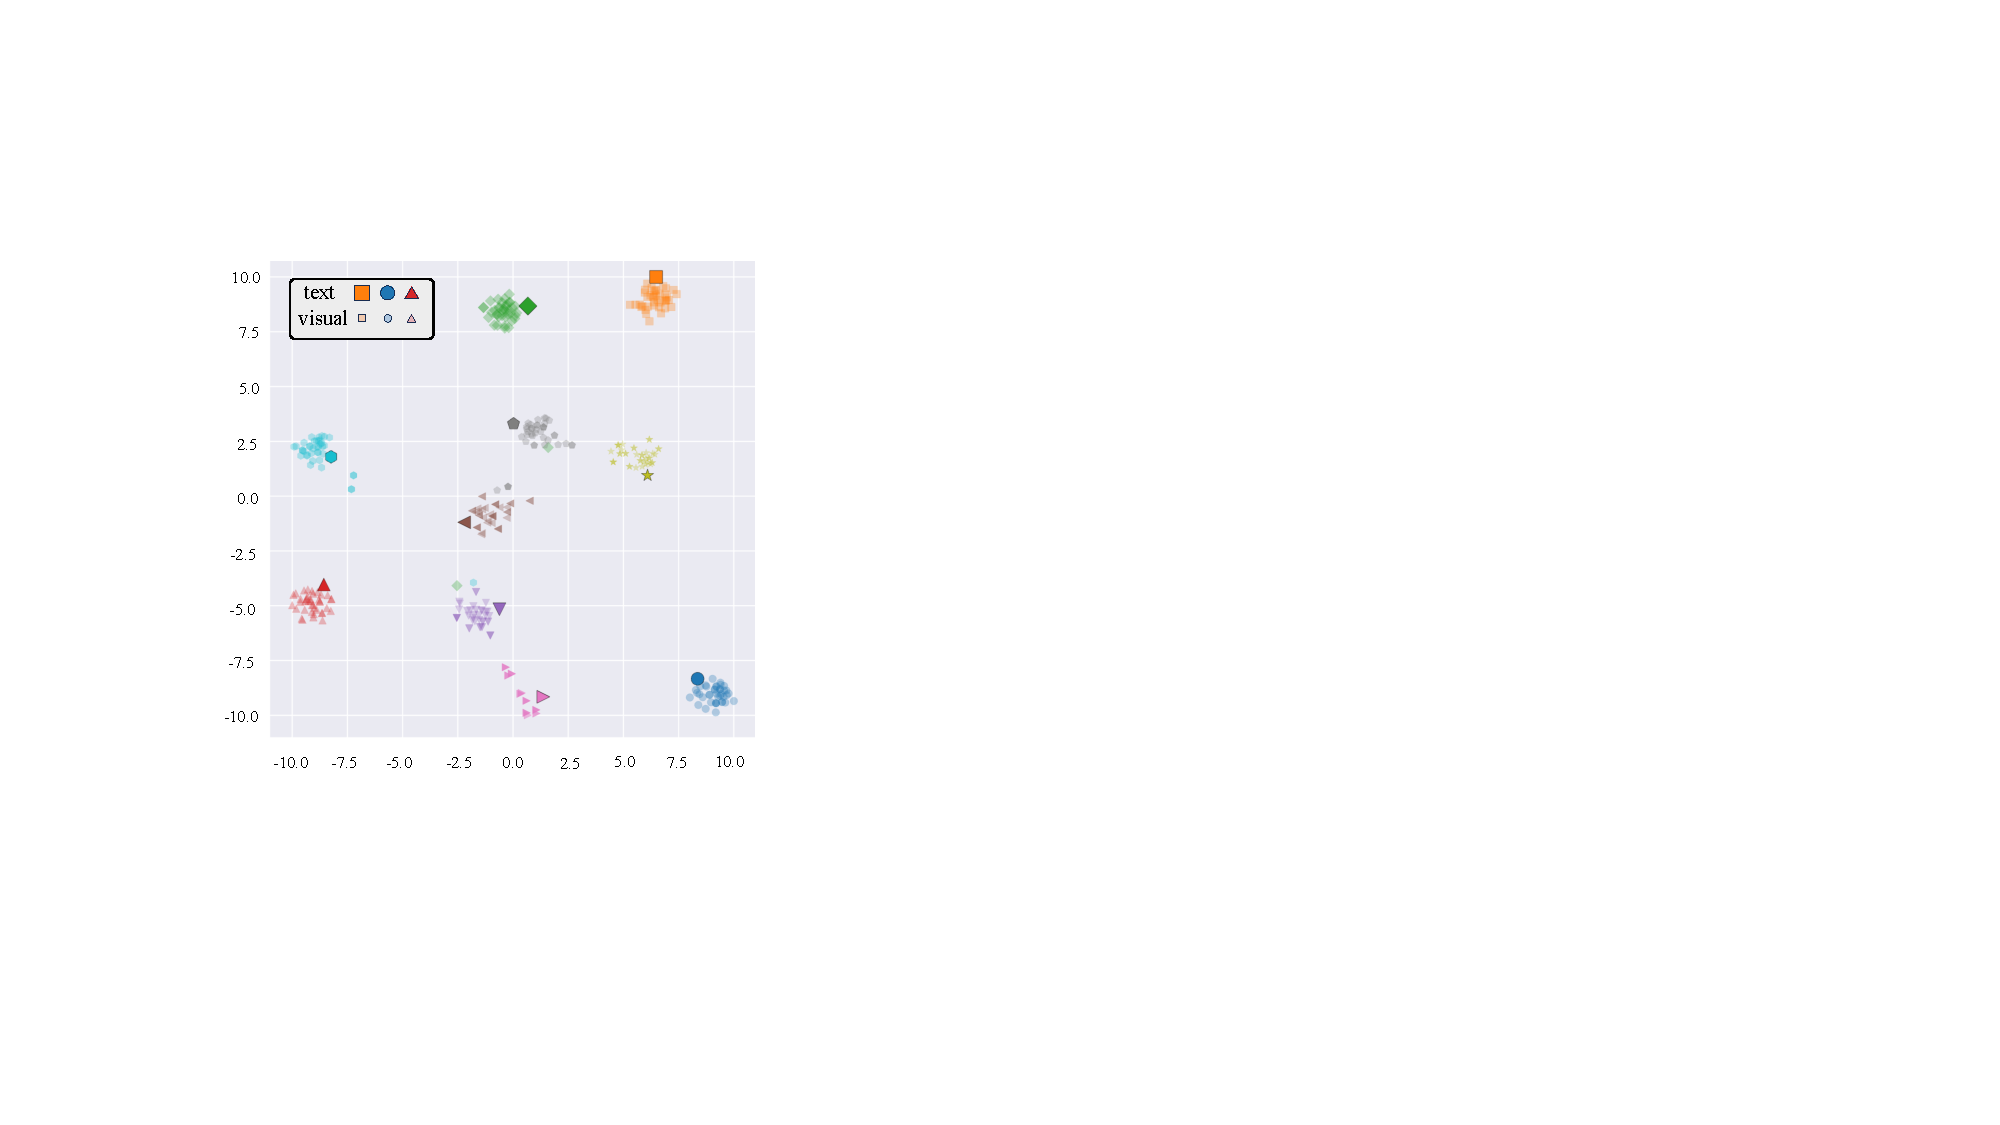
\includegraphics[width=\textwidth]{images/tsne_align.pdf}
    \caption{w/ contrastive align}
    \label{fig:tsne_align}
\end{subfigure}
\caption{t-SNE~\cite{van2008visualizing} visualization of text prompt and visual prompt embeddings. We pick the first 10 categories in COCO training set and randomly sample 30 images for each category to get visual prompts.}
\vspace{-1em}
\label{fig:combined}
\end{figure}

\begin{table}[]
  \centering
  \resizebox{\columnwidth}{!}{%
    \begin{tabular}{c|c|c|cccc}
  \hline
  \multirow{2}{*}{\begin{tabular}[c]{@{}c@{}}Training\\ Strategy\end{tabular}}         & \multirow{2}{*}{\begin{tabular}[c]{@{}c@{}}Prompt\\ Type\end{tabular}} & \begin{tabular}[c]{@{}c@{}}COCO-Val\\ Zero-Shot\end{tabular} & \multicolumn{4}{c}{\begin{tabular}[c]{@{}c@{}}LVIS-Val\\ Zero-Shot\end{tabular}} \\ \cline{3-7} 
                                                                                       &                                                                        & AP                                                           & AP                                  & $AP_r$                               & $AP_c$                                            & $AP_f$              \\ \hline
  Text Prompt Only                                                                     & Text                                                                   & 46.4                                                         & 32.8                                & 32.1                               & 32.0                                            & 34.0              \\
  Visual Prompt Only                                                                   & Visual-G                                                               & 14.0                                                         & 15.3                                & 8.6                                & 11.3                                            & 22.8              \\ \hline
  \multirow{2}{*}{\begin{tabular}[c]{@{}c@{}}W/O Contrastive\\ Alignment\end{tabular}} & Text                                                                   & 44.4                                                         & 32.2                                & 28.2                               & 28.9                                            & 37.6              \\
                                                                                       & Visual-G                                                               & 38.7                                                         & 30.2                                & 29.4                               & 26.9                                            & 38.7              \\ \hline
  \multirow{2}{*}{\begin{tabular}[c]{@{}c@{}}W/ Contrastive\\ Alignment\end{tabular}}  & Text                                                                   & 45.8\textcolor{deepgreen}{(+1.4)}                            & 34.8\textcolor{deepgreen}{(+2.6)}   & 29.0\textcolor{deepgreen}{(+0.8)}  & 31.5\textcolor{deepgreen}{(+2.6)}               & 41.2\textcolor{deepgreen}{(+3.6)}               \\
                                                                                       & Visual-G                                                               & 38.8\textcolor{deepgreen}{(+0.1)}                            & 34.9\textcolor{deepgreen}{(+4.7)}   & 32.4\textcolor{deepgreen}{(+3.0)}  & 30.3\textcolor{deepgreen}{(+3.4)}               & 41.1\textcolor{deepgreen}{(+2.4)}               \\ \hline
  \end{tabular}}
\caption{Ablationon the proposed text-visual synergy.}
\label{tab:synergy_ab}
\end{table}

\begin{table}[]
  \centering
  \resizebox{\columnwidth}{!}{%
    \begin{tabular}{cc|c|cccc}
\hline
\multirow{2}{*}{\# Prompts} & \multirow{2}{*}{\begin{tabular}[c]{@{}c@{}}Prompt \\ Type\end{tabular}} & \begin{tabular}[c]{@{}c@{}}COCO-Val\\ Zero-Shot\end{tabular} & \multicolumn{4}{c}{\begin{tabular}[c]{@{}c@{}}LVIS-Val\\ Zero-Shot\end{tabular}} \\ \cline{3-7} 
                            &                                                                         & AP                                                           & AP                 & $AP_r$               & $AP_c$               & $AP_f$              \\ \hline
1                           & Visual-G                                                                & 29.2                                                         & 26.2               & 27.6               & 21.3               & 30.9              \\
4                           & Visual-G                                                                & 32.9                                                         & 32.9               & 32.0               & 28.2               & 38.7              \\
16                          & Visual-G                                                                & 38.8                                                         & 34.9               & 32.4               & 30.3               & 41.1              \\
32                          & Visual-G                                                                & 41.3                                                         & 35.1               & 32.2               & 30.3               & 41.7              \\
64                          & Visual-G                                                                & 41.4                                                         & 35.2               & 32.4               & 30.4               & 41.8              \\ \hline
\end{tabular}
  } 
\caption{Ablation experiments on the number of visual prompts and their generic object detection capabilities}
\label{tab:num_visual_promtps}
\end{table}

\begin{table*}[h]
    \resizebox{\linewidth}{!}{
      \begin{tabular}{cc|c|l|c|cccc}
\hline
\multirow{2}{*}{Model} & \multirow{2}{*}{\begin{tabular}[c]{@{}c@{}}Prompt\\ Type\end{tabular}} & \multirow{2}{*}{\begin{tabular}[c]{@{}c@{}}Training\\ Data\end{tabular}} & \multirow{2}{*}{\begin{tabular}[c]{@{}l@{}}Data\\ Size\end{tabular}} & \begin{tabular}[c]{@{}c@{}}COCO-Val\\ Zero-Shot\end{tabular} & \multicolumn{4}{c}{\begin{tabular}[c]{@{}c@{}}LVIS-Minival\\ Zero-Shot\end{tabular}} \\ \cline{5-9} 
                       &                                                                        &                                                                          &                                                                      & AP                                                           & AP             & AP-R            & AP-C          & AP-F                              \\ \hline
Grounding DINO-T       & Text                                                                   & O365, GoldG                                                              & 1.4M                                                                 & 48.1                                                         & 25.6           & 14.14           & 19.6          & 32.2                              \\
Grounding DINO-T       & Text                                                                   & O365, GoldG, Cap4M                                                       & 5.4M                                                                 & 48.4                                                         & 27.4           & 18.1            & 23.3          & 32.7                              \\ \hline
T-Rex2-T               & Text                                                                   & O365, GoldG                                                              & 1.4M                                                                 & 46.1                                                         & 34.9           & 32.7            & 32.9          & 37.1                              \\
T-Rex2-T               & Text                                                                   & O365, GoldG, Bamboo                                                      & 2.5M                                                                 & 45.7                                                         & 38.7           & 35.3            & 39.4          & 38.8                              \\
T-Rex2-T               & Text                                                                   & O365, GoldG, OpenImages, Bamboo, CC3M, LAION                             & 6.5M                                                                 & 46.4                                                         & 39.3           & 35.4            & 40.5          & 39.0                              \\ \hline
T-Rex2-T               & Visual-G                                                               & O365, OpenImages, HierText, CrowdHuman                                   & \multicolumn{1}{c|}{2.4M}                                            & 41.1                                                            & 38.1              & 25.8               & 34.4             & 43.7                                 \\
T-Rex2-T               & Visual-G                                                               & O365, OpenImages, HierText, CrowdHuman, SA-1B                            & \multicolumn{1}{c|}{3.1M}                                            & 38.8                                                         & 37.4           & 29.9            & 33.9          & 41.8                              \\ \hline
T-Rex2-T               & Visual-I (Box)                                                         & O365, OpenImages, HierText, CrowdHuman                                   & \multicolumn{1}{c|}{2.4M}                                            & 41.1                                                         & 40.6           & 40.3            & 43.5          & \multicolumn{1}{l}{38.1}          \\
T-Rex2-T               & Visual-I (Box)                                                         & O365, OpenImages, HierText, CrowdHuman, SA-1B                            & \multicolumn{1}{c|}{3.1M}                                            & 56.6                                                         & 59.3           & 64.4            & 63.5          & \multicolumn{1}{l}{54.6}          \\ \hline
\end{tabular}}
    \caption{Ablation of the proposed data engines.}
    \label{tab:data_engine}
    \end{table*}

\noindent\textbf{Ablations of contrastive alignment.}
As presented in Tab. \ref{tab:synergy_ab} (last two rows), employing contrastive alignment can lead to improved performance for both text and visual prompts. With contrastive alignment, the distribution between text prompt and visual prompt is more structured as shown in Fig. \ref{fig:tsne_align}: text prompts act as anchors and visual prompts cluster around them. This distribution means that visual prompts can learn or derive general knowledge from the closely associated text prompt, making the learning process more efficient. Furthermore, the text prompts are more separated in the feature space compared to Fig. \ref{fig:tsne_noalign}, this indicates that it allows for refinement of text prompts by exposing them to a vast array of visual prompts, thus making them more unique and better defined.


\noindent\textbf{Ablation of generic visual prompt.} In Tab. \ref{tab:num_visual_promtps}, we show that by using more visual prompts, the generic detection capability can be gradually increased. The reason is that visual prompts are not as versatile as text prompts, so we need a large number of visual examples to characterize a generic concept as well as possible. 

\noindent\textbf{Ablation of mixed prompt.}  We further show the results of mixed prompts for generic object detection. This hybrid method aims to leverage the strengths of both modalities to improve detection performance. In Tab. \ref{tab:joint_inference}, the mixed prompt on COCO achieves a result that is balanced between text prompt and visual prompt, while on LVIS there is a further performance improvement. We believe that this hybrid inference workflow is more suitable for the case of long-tailed distributions, where text prompt and visual prompt can promote each other. 

\noindent\textbf{Ablation of data engines.} In Tab. \ref{tab:data_engine}, we ablate the effectiveness of the two data engines. For text prompts, introducing the Bamboo dataset improves the performance on the LVIS dataset (+3.8AP), owing to its diverse categories, but slightly declined performance on the COCO dataset (-0.4AP), indicating that the model is less fitted to COCO categories. Adding image caption data further improves the performance on both benchmarks. For visual prompts, the introduction of the SA-1B data significantly improves the interactive capability of the model, but slightly weakens its generic capability. We speculate that the observed performance degradation may stem from the inadequacy of simply employing TAP~\cite{pan2023tokenize} for object classification within SA-1B, which results in incorrect semantic learning by the model on the SA-1B data. Future work will entail further optimization of this data engine.

\noindent\textbf{Ablation of inference speed.}
In this section, we measure the inference speed of each module of T-Rex2. The experiment is conducted on an NVIDIA RTX 3090 GPU with a batch size of 1. Before measurement, we conducted a warm-up phase to stabilize GPU performance. Inference times were recorded over 100 iterations. The results are shown in Tab. \ref{tab:speed}. Benefiting from the late fusion design, \ourmodel{} can work in real-time when using the interactive visual prompt mode. Specifically, after a user uploads a picture, we only need to process it once with our main processing steps (backbone and encoder) to get the image features. Any further interactions from the user involve just running our visual prompt encoder and decoder multiple times, which is in a real-time manner. This quick response is especially useful for scenarios like automatic annotation.

\begin{table}[]
  \centering
  \resizebox{\columnwidth}{!}{%
    \begin{tabular}{c|ccccc|c|c}
\hline
Backbone & backbone & encoder & \begin{tabular}[c]{@{}c@{}}visual prompt \\ encoder\end{tabular} & \begin{tabular}[c]{@{}c@{}}text prompt \\ encoder\end{tabular} & decoder & FPS   & \begin{tabular}[c]{@{}c@{}}Interactive\\  FPS\end{tabular} \\ \hline
Swin-T   & 0.0318   & 0.0240  & 0.0120                                                           & 0.0103                                                         & 0.0180  & 10.41 & 33.33                                                      \\
Swin-L   & 0.1220   & 0.0929  & 0.0261                                                           & 0.0116                                                         & 0.0240  & 3.62  & 19.96                                                      \\ \hline
\end{tabular}}
\caption{Time cost for each module in \ourmodel{}. Interactive FPS is the inference speed of the visual prompt encoder and the decoder. Since \ourmodel{} is a late fusion model, we only need to forward the backbone and encoder for once, and multi-round interactions only require running the prompt encoder and decoder.}
\label{tab:speed}
\end{table}

\begin{table}[]
\centering
\resizebox{0.8\columnwidth}{!}{%
\begin{tabular}{c|c|cccc}
\hline
\multirow{2}{*}{\begin{tabular}[c]{@{}c@{}}prompt\\ combination\end{tabular}} & \begin{tabular}[c]{@{}c@{}}COCO-Val\\ Zero-Shot\end{tabular} & \multicolumn{4}{c}{\begin{tabular}[c]{@{}c@{}}LVIS-Val\\ Zero-Shot\end{tabular}} \\ \cline{2-6} 
                                                                              & AP                                                           & AP                 & $AP_r$               & $AP_c$               & $AP_f$              \\ \hline
Text                                                                        & \textbf{45.8}                                                & 34.8               & 29.0               & 31.5               & 41.2              \\ \hline
Visual-G                                                                   & 38.8                                                         & 34.9               & 32.4               & 30.3               & 41.1              \\ \hline
\begin{tabular}[c]{@{}c@{}}Text + \\ Visual-G\end{tabular}               & 42.5                                                         & \textbf{37.0}      & \textbf{34.3}      & \textbf{33.8}      & \textbf{41.7}     \\ \hline
\end{tabular}
  }
\caption{Zero-shot object detection results on mixed prompt mode.}
\label{tab:joint_inference}
\end{table}



\section{Conclusion}
\ourmodel{} is a promising attempt towards generic object detection. We reveal the complementary advantages between text prompts and visual prompts, and successfully align the two prompt modalities into a single model, making it both generic and interactive for open-set object detection. We show that these two prompt modalities can benefit from each other and gain performance through contrastive learning. By switching between different prompt modalities in different scenarios, \ourmodel{} demonstrates impressive zero-shot object detection capabilities and can be used in a variety of applications. We hope that this work will bring new insights into the field of open-set object detection and contribute to further development.

\textbf{Limitations. }Despite the integration of text and visual prompts showing mutual benefits within a unified model, challenges arise. Visual prompts may sometimes interfere with text prompts, especially in scenarios involving common objects, as indicated by the reduced performance on the COCO benchmark when both are used together in Tab. \ref{tab:joint_inference}. Despite this, improvements on the LVIS benchmark highlight the potential benefits of this approach. Therefore, further research into improving the alignment between these modalities is essential. Moreover, the requirement for up to 16 visual examples to ensure reliable detection due to visual diversity highlights a need for methods that enable visual prompts to achieve similar effectiveness with fewer visual examples.

\section*{Acknowledgments}
We would like to thank everyone involved in the T-Rex2 project, including project lead Lei Zhang, application lead Wei Liu, product manager Qin Liu and Xiaohui Wang, front-end developers Yuanhao Zhu, Ce Feng, and Jiongrong Fan, back-end developers Weiqiang Hu and Zhiqiang Li, UX designer Xinyi Ruan, and tester Yinuo Chen.